% % % % % % % % % % % % % % % % % % % % % % % % % % % % % % % % % % % % % % IV
\section{Coherence}

\begin{frame}
  \begin{block}{Coherence}
    In simple worlds, \emph{coherence} is a state or measure of some \emph{pieces}
    fitting together into a whole. Coherence can be applied to almost any aspect of
    the universe.
  \end{block}
  \begin{quote}
    The consistency or \emph{coherence} within a logical or mathematical
    system, means that $p$ and $\neg p$ must not be derivable from the
    basic assumptions in accordance with the observance of the syntactical
    rules (Daya, 1960).
  \end{quote}
  \begin{quote}
    Coherence theory is a psychologically motivated motivational cognitive theory with
    foundations in philosophy that approaches problems in terms of the satisfaction
    of multiple constraints within networks of highly interconnected elements
    (Sindhu, 2010).
  \end{quote}
\end{frame}


\begin{frame}{Coherence}
  \begin{block}{Coherence by Thagard}
    Thagard (1998) claimed that \alert{coherence} can be understood in terms of
    \alert{maximal satisfaction of multiple constraints}.

    \medskip
    By Thagard, coherence problem is about \underline{partitioning a graph} of
    \emph{information pieces}, interconnected by positive or negative weighted
    constraints, that enhance or diminish partition's coherence.
  \end{block}
\end{frame}
\begin{frame}{Coherence}
  \begin{block}{Information Graph Splitting}
    The information graph $\mathcal{V}$ consists of
    classes $C_1,\dots,C_4$, also there are three possibilities for
    class $C_1$ placement and two for class $C_4$.\\\bigskip
    \begin{columns}
      \begin{column}{.3\textwidth}
        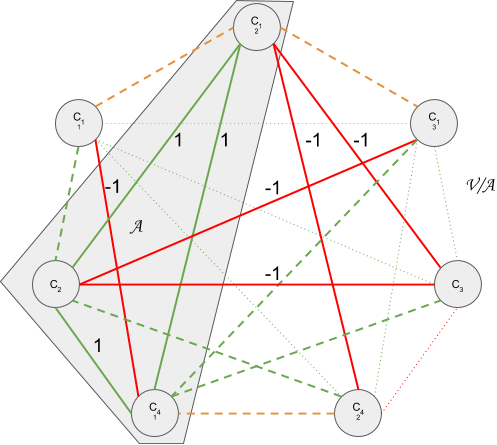
\includegraphics[width=\textwidth, trim={20pt 20pt 100pt 20pt}]
                        {\rootdir/img/UAB-splitting.png}
      \end{column}
      \begin{column}{.8\textwidth}
        \qquad\quad A relation is
        \begin{mdframed}[leftmargin=2cm, hidealllines=true]
          \begin{itemize}
            \item[\red{\emph{inconsistent}}], if two classes intersect in time;
            \item[\yellow{\emph{same class}}], if two classes differ only by time;
            \item[\green{\emph{consistent}}], otherwise.
          \end{itemize}
        \end{mdframed}
      \end{column}
    \end{columns}
  \end{block}
\end{frame}

% % % % % % % % % % % % % % % % % % % %
\subsection{Contexts}

\begin{frame}{Coherence}
  \begin{block}{Contexts}
    Describe aspects of coherence problem.
    \begin{columns}[t]
      \begin{column}{.5\textwidth}
        \begin{block}{Original}
          Proposed by Sindhu (2010) \\\medskip
          \begin{itemize}
            \item Contexts represent BDI
            \item Each context has own logic
            \item Contexts are connected by
                  \emph{bridge rules}
          \end{itemize}
        \end{block}
      \end{column}
      \begin{column}{.5\textwidth}
        \begin{block}{Proposed}
          \begin{itemize}
            \item Contexts represent groups of constraints
            \item \underline{Assess coherence}
                  of the given information and tell whether
                  it is \underline{coherent}
            \item Candidate is \alert{\underline{propagated}} through
                  the contexts
          \end{itemize}
        \end{block}
      \end{column}
    \end{columns}
  \end{block}
\end{frame}

\againframe{constraints}

\begin{frame}{Contexts}
  \begin{columns}
    \begin{column}{.2\textwidth}\end{column}
    \begin{column}{.2\textwidth}
      \tikz\draw[->, >=stealth, double, thick]
                (0,0)  node[yshift=10pt] {Candidate $\tilde{c}$}
                  --
                (0,-5) node[yshift=-10pt] {Assessed candidate $\tilde{c}$};
    \end{column}
    \begin{column}{.5\textwidth}
      \vfill
      \begin{enumerate}
        \item Common / Independent
          \begin{enumerate}
            \item Class constraints
            \item Time constraints
          \end{enumerate}
        \item Internal / Personal
          \begin{enumerate}
            \item Obligations (strong)
            \item Preferences (weak)
          \end{enumerate}
        \item \underline{External}\\
              communicates, works towards
              \emph{common goal}
      \end{enumerate}
      \vfill
    \end{column}
    \begin{column}{.3\textwidth}\end{column}
  \end{columns}
\end{frame}
